\documentclass[1p]{elsarticle_modified}
%\bibliographystyle{elsarticle-num}

%\usepackage[colorlinks]{hyperref}
%\usepackage{abbrmath_seonhwa} %\Abb, \Ascr, \Acal ,\Abf, \Afrak
\usepackage{amsfonts}
\usepackage{amssymb}
\usepackage{amsmath}
\usepackage{amsthm}
\usepackage{scalefnt}
\usepackage{amsbsy}
\usepackage{kotex}
\usepackage{caption}
\usepackage{subfig}
\usepackage{color}
\usepackage{graphicx}
\usepackage{xcolor} %% white, black, red, green, blue, cyan, magenta, yellow
\usepackage{float}
\usepackage{setspace}
\usepackage{hyperref}

\usepackage{tikz}
\usetikzlibrary{arrows}

\usepackage{multirow}
\usepackage{array} % fixed length table
\usepackage{hhline}

%%%%%%%%%%%%%%%%%%%%%
\makeatletter
\renewcommand*\env@matrix[1][\arraystretch]{%
	\edef\arraystretch{#1}%
	\hskip -\arraycolsep
	\let\@ifnextchar\new@ifnextchar
	\array{*\c@MaxMatrixCols c}}
\makeatother %https://tex.stackexchange.com/questions/14071/how-can-i-increase-the-line-spacing-in-a-matrix
%%%%%%%%%%%%%%%

\usepackage[normalem]{ulem}

\newcommand{\msout}[1]{\ifmmode\text{\sout{\ensuremath{#1}}}\else\sout{#1}\fi}
%SOURCE: \msout is \stkout macro in https://tex.stackexchange.com/questions/20609/strikeout-in-math-mode

\newcommand{\cancel}[1]{
	\ifmmode
	{\color{red}\msout{#1}}
	\else
	{\color{red}\sout{#1}}
	\fi
}

\newcommand{\add}[1]{
	{\color{blue}\uwave{#1}}
}

\newcommand{\replace}[2]{
	\ifmmode
	{\color{red}\msout{#1}}{\color{blue}\uwave{#2}}
	\else
	{\color{red}\sout{#1}}{\color{blue}\uwave{#2}}
	\fi
}

\newcommand{\Sol}{\mathcal{S}} %segment
\newcommand{\D}{D} %diagram
\newcommand{\A}{\mathcal{A}} %arc


%%%%%%%%%%%%%%%%%%%%%%%%%%%%%5 test

\def\sl{\operatorname{\textup{SL}}(2,\Cbb)}
\def\psl{\operatorname{\textup{PSL}}(2,\Cbb)}
\def\quan{\mkern 1mu \triangleright \mkern 1mu}

\theoremstyle{definition}
\newtheorem{thm}{Theorem}[section]
\newtheorem{prop}[thm]{Proposition}
\newtheorem{lem}[thm]{Lemma}
\newtheorem{ques}[thm]{Question}
\newtheorem{cor}[thm]{Corollary}
\newtheorem{defn}[thm]{Definition}
\newtheorem{exam}[thm]{Example}
\newtheorem{rmk}[thm]{Remark}
\newtheorem{alg}[thm]{Algorithm}

\newcommand{\I}{\sqrt{-1}}
\begin{document}

%\begin{frontmatter}
%
%\title{Boundary parabolic representations of knots up to 8 crossings}
%
%%% Group authors per affiliation:
%\author{Yunhi Cho} 
%\address{Department of Mathematics, University of Seoul, Seoul, Korea}
%\ead{yhcho@uos.ac.kr}
%
%
%\author{Seonhwa Kim} %\fnref{s_kim}}
%\address{Center for Geometry and Physics, Institute for Basic Science, Pohang, 37673, Korea}
%\ead{ryeona17@ibs.re.kr}
%
%\author{Hyuk Kim}
%\address{Department of Mathematical Sciences, Seoul National University, Seoul 08826, Korea}
%\ead{hyukkim@snu.ac.kr}
%
%\author{Seokbeom Yoon}
%\address{Department of Mathematical Sciences, Seoul National University, Seoul, 08826,  Korea}
%\ead{sbyoon15@snu.ac.kr}
%
%\begin{abstract}
%We find all boundary parabolic representation of knots up to 8 crossings.
%
%\end{abstract}
%\begin{keyword}
%    \MSC[2010] 57M25 
%\end{keyword}
%
%\end{frontmatter}

%\linenumbers
%\tableofcontents
%
\newcommand\colored[1]{\textcolor{white}{\rule[-0.35ex]{0.8em}{1.4ex}}\kern-0.8em\color{red} #1}%
%\newcommand\colored[1]{\textcolor{white}{ #1}\kern-2.17ex	\textcolor{white}{ #1}\kern-1.81ex	\textcolor{white}{ #1}\kern-2.15ex\color{red}#1	}

{\Large $\underline{12a_{0837}~(K12a_{0837})}$}

\setlength{\tabcolsep}{10pt}
\renewcommand{\arraystretch}{1.6}
\vspace{1cm}\begin{tabular}{m{100pt}>{\centering\arraybackslash}m{274pt}}
\multirow{5}{120pt}{
	\centering
	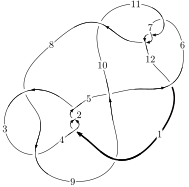
\includegraphics[width=112pt]{../../../GIT/diagram.site/Diagrams/png/1638_12a_0837.png}\\
\ \ \ A knot diagram\footnotemark}&
\allowdisplaybreaks
\textbf{Linearized knot diagam} \\
\cline{2-2}
 &
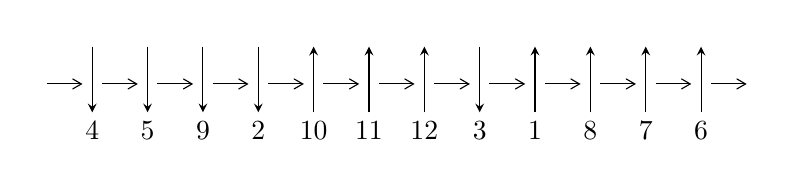
\begin{tikzpicture}[x=20pt, y=17pt]
	% nodes
	\node (C0) at (0, 0) {};
	\node (C1) at (1, 0) {};
	\node (C1U) at (1, +1) {};
	\node (C1D) at (1, -1) {4};

	\node (C2) at (2, 0) {};
	\node (C2U) at (2, +1) {};
	\node (C2D) at (2, -1) {5};

	\node (C3) at (3, 0) {};
	\node (C3U) at (3, +1) {};
	\node (C3D) at (3, -1) {9};

	\node (C4) at (4, 0) {};
	\node (C4U) at (4, +1) {};
	\node (C4D) at (4, -1) {2};

	\node (C5) at (5, 0) {};
	\node (C5U) at (5, +1) {};
	\node (C5D) at (5, -1) {10};

	\node (C6) at (6, 0) {};
	\node (C6U) at (6, +1) {};
	\node (C6D) at (6, -1) {11};

	\node (C7) at (7, 0) {};
	\node (C7U) at (7, +1) {};
	\node (C7D) at (7, -1) {12};

	\node (C8) at (8, 0) {};
	\node (C8U) at (8, +1) {};
	\node (C8D) at (8, -1) {3};

	\node (C9) at (9, 0) {};
	\node (C9U) at (9, +1) {};
	\node (C9D) at (9, -1) {1};

	\node (C10) at (10, 0) {};
	\node (C10U) at (10, +1) {};
	\node (C10D) at (10, -1) {8};

	\node (C11) at (11, 0) {};
	\node (C11U) at (11, +1) {};
	\node (C11D) at (11, -1) {7};

	\node (C12) at (12, 0) {};
	\node (C12U) at (12, +1) {};
	\node (C12D) at (12, -1) {6};
	\node (C13) at (13, 0) {};

	% arrows
	\draw[->,>={angle 60}]
	(C0) edge (C1) (C1) edge (C2) (C2) edge (C3) (C3) edge (C4) (C4) edge (C5) (C5) edge (C6) (C6) edge (C7) (C7) edge (C8) (C8) edge (C9) (C9) edge (C10) (C10) edge (C11) (C11) edge (C12) (C12) edge (C13) ;	\draw[->,>=stealth]
	(C1U) edge (C1D) (C2U) edge (C2D) (C3U) edge (C3D) (C4U) edge (C4D) (C5D) edge (C5U) (C6D) edge (C6U) (C7D) edge (C7U) (C8U) edge (C8D) (C9D) edge (C9U) (C10D) edge (C10U) (C11D) edge (C11U) (C12D) edge (C12U) ;
	\end{tikzpicture} \\
\hhline{~~} \\& 
\textbf{Solving Sequence} \\ \cline{2-2} 
 &
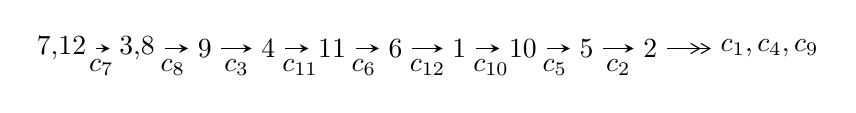
\begin{tikzpicture}[x=23pt, y=7pt]
	% node
	\node (A0) at (-1/8, 0) {7,12};
	\node (A1) at (17/16, 0) {3,8};
	\node (A2) at (17/8, 0) {9};
	\node (A3) at (25/8, 0) {4};
	\node (A4) at (33/8, 0) {11};
	\node (A5) at (41/8, 0) {6};
	\node (A6) at (49/8, 0) {1};
	\node (A7) at (57/8, 0) {10};
	\node (A8) at (65/8, 0) {5};
	\node (A9) at (73/8, 0) {2};
	\node (C1) at (1/2, -1) {$c_{7}$};
	\node (C2) at (13/8, -1) {$c_{8}$};
	\node (C3) at (21/8, -1) {$c_{3}$};
	\node (C4) at (29/8, -1) {$c_{11}$};
	\node (C5) at (37/8, -1) {$c_{6}$};
	\node (C6) at (45/8, -1) {$c_{12}$};
	\node (C7) at (53/8, -1) {$c_{10}$};
	\node (C8) at (61/8, -1) {$c_{5}$};
	\node (C9) at (69/8, -1) {$c_{2}$};
	\node (A10) at (11, 0) {$c_{1},c_{4},c_{9}$};

	% edge
	\draw[->,>=stealth]	
	(A0) edge (A1) (A1) edge (A2) (A2) edge (A3) (A3) edge (A4) (A4) edge (A5) (A5) edge (A6) (A6) edge (A7) (A7) edge (A8) (A8) edge (A9) ;
	\draw[->>,>={angle 60}]	
	(A9) edge (A10);
\end{tikzpicture} \\ 

\end{tabular} \\

\footnotetext{
The image of knot diagram is generated by the software ``\textbf{Draw programme}" developed by Andrew Bartholomew(\url{http://www.layer8.co.uk/maths/draw/index.htm\#Running-draw}), where we modified some parts for our purpose(\url{https://github.com/CATsTAILs/LinksPainter}).
}\phantom \\ \newline 
\centering \textbf{Ideals for irreducible components\footnotemark of $X_{\text{par}}$} 
 
\begin{align*}
I^u_{1}&=\langle 
u^{78}-30 u^{76}+\cdots+b-2 u,\;- u^{78}- u^{77}+\cdots+a+2,\;u^{80}+2 u^{79}+\cdots-4 u+1\rangle \\
I^u_{2}&=\langle 
- u^7+2 u^5+u^4- u^3- u^2+b- u,\;u^7- u^6-2 u^5+2 u^4+u^3- u^2+a+u-1,\\
\phantom{I^u_{2}}&\phantom{= \langle  }u^8- u^7-3 u^6+2 u^5+3 u^4-2 u-1\rangle \\
\\
\end{align*}
\raggedright * 2 irreducible components of $\dim_{\mathbb{C}}=0$, with total 88 representations.\\
\footnotetext{All coefficients of polynomials are rational numbers. But the coefficients are sometimes approximated in decimal forms when there is not enough margin.}
\newpage
\renewcommand{\arraystretch}{1}
\centering \section*{I. $I^u_{1}= \langle u^{78}-30 u^{76}+\cdots+b-2 u,\;- u^{78}- u^{77}+\cdots+a+2,\;u^{80}+2 u^{79}+\cdots-4 u+1 \rangle$}
\flushleft \textbf{(i) Arc colorings}\\
\begin{tabular}{m{7pt} m{180pt} m{7pt} m{180pt} }
\flushright $a_{7}=$&$\begin{pmatrix}1\\0\end{pmatrix}$ \\
\flushright $a_{12}=$&$\begin{pmatrix}0\\u\end{pmatrix}$ \\
\flushright $a_{3}=$&$\begin{pmatrix}u^{78}+u^{77}+\cdots-5 u-2\\- u^{78}+30 u^{76}+\cdots+2 u^2+2 u\end{pmatrix}$ \\
\flushright $a_{8}=$&$\begin{pmatrix}1\\- u^2\end{pmatrix}$ \\
\flushright $a_{9}=$&$\begin{pmatrix}u^{15}-6 u^{13}+14 u^{11}-14 u^9+2 u^7+6 u^5-2 u^3-2 u\\- u^{15}+5 u^{13}-8 u^{11}+u^9+8 u^7-4 u^5-2 u^3+u\end{pmatrix}$ \\
\flushright $a_{4}=$&$\begin{pmatrix}u^{78}+u^{77}+\cdots- u-3\\2 u^{79}+u^{78}+\cdots-7 u+2\end{pmatrix}$ \\
\flushright $a_{11}=$&$\begin{pmatrix}- u\\u\end{pmatrix}$ \\
\flushright $a_{6}=$&$\begin{pmatrix}- u^2+1\\u^2\end{pmatrix}$ \\
\flushright $a_{1}=$&$\begin{pmatrix}u^5-2 u^3+u\\- u^5+u^3+u\end{pmatrix}$ \\
\flushright $a_{10}=$&$\begin{pmatrix}u^3-2 u\\- u^5+u^3+u\end{pmatrix}$ \\
\flushright $a_{5}=$&$\begin{pmatrix}u^{10}-5 u^8+8 u^6-3 u^4-3 u^2+1\\- u^{12}+4 u^{10}-4 u^8-2 u^6+3 u^4+2 u^2\end{pmatrix}$ \\
\flushright $a_{2}=$&$\begin{pmatrix}u^{78}+u^{77}+\cdots-2 u-2\\u^{79}-32 u^{77}+\cdots-2 u+1\end{pmatrix}$\\&\end{tabular}
\flushleft \textbf{(ii) Obstruction class $= -1$}\\~\\
\flushleft \textbf{(iii) Cusp Shapes $= -3 u^{79}+98 u^{77}+\cdots-2 u-11$}\\~\\
\newpage\renewcommand{\arraystretch}{1}
\flushleft \textbf{(iv) u-Polynomials at the component}\newline \\
\begin{tabular}{m{50pt}|m{274pt}}
Crossings & \hspace{64pt}u-Polynomials at each crossing \\
\hline $$\begin{aligned}c_{1},c_{2},c_{4}\end{aligned}$$&$\begin{aligned}
&u^{80}-9 u^{79}+\cdots+6 u-1
\end{aligned}$\\
\hline $$\begin{aligned}c_{3},c_{8}\end{aligned}$$&$\begin{aligned}
&u^{80}+u^{79}+\cdots-384 u-256
\end{aligned}$\\
\hline $$\begin{aligned}c_{5}\end{aligned}$$&$\begin{aligned}
&u^{80}+2 u^{79}+\cdots+1220 u+757
\end{aligned}$\\
\hline $$\begin{aligned}c_{6},c_{7},c_{11}\end{aligned}$$&$\begin{aligned}
&u^{80}-2 u^{79}+\cdots+4 u+1
\end{aligned}$\\
\hline $$\begin{aligned}c_{9}\end{aligned}$$&$\begin{aligned}
&u^{80}-6 u^{79}+\cdots+123136 u-10736
\end{aligned}$\\
\hline $$\begin{aligned}c_{10},c_{12}\end{aligned}$$&$\begin{aligned}
&u^{80}+6 u^{79}+\cdots-292 u-53
\end{aligned}$\\
\hline
\end{tabular}\\~\\
\newpage\renewcommand{\arraystretch}{1}
\flushleft \textbf{(v) Riley Polynomials at the component}\newline \\
\begin{tabular}{m{50pt}|m{274pt}}
Crossings & \hspace{64pt}Riley Polynomials at each crossing \\
\hline $$\begin{aligned}c_{1},c_{2},c_{4}\end{aligned}$$&$\begin{aligned}
&y^{80}-79 y^{79}+\cdots+20 y+1
\end{aligned}$\\
\hline $$\begin{aligned}c_{3},c_{8}\end{aligned}$$&$\begin{aligned}
&y^{80}-51 y^{79}+\cdots-638976 y+65536
\end{aligned}$\\
\hline $$\begin{aligned}c_{5}\end{aligned}$$&$\begin{aligned}
&y^{80}+6 y^{79}+\cdots+12140628 y+573049
\end{aligned}$\\
\hline $$\begin{aligned}c_{6},c_{7},c_{11}\end{aligned}$$&$\begin{aligned}
&y^{80}-66 y^{79}+\cdots-24 y+1
\end{aligned}$\\
\hline $$\begin{aligned}c_{9}\end{aligned}$$&$\begin{aligned}
&y^{80}+42 y^{79}+\cdots-4371656480 y+115261696
\end{aligned}$\\
\hline $$\begin{aligned}c_{10},c_{12}\end{aligned}$$&$\begin{aligned}
&y^{80}+54 y^{79}+\cdots-91836 y+2809
\end{aligned}$\\
\hline
\end{tabular}\\~\\
\newpage\flushleft \textbf{(vi) Complex Volumes and Cusp Shapes}
$$\begin{array}{c|c|c}  
\text{Solutions to }I^u_{1}& \I (\text{vol} + \sqrt{-1}CS) & \text{Cusp shape}\\
 \hline 
\begin{aligned}
u &= -0.876291 + 0.160225 I \\
a &= \phantom{-}0.126511 + 0.194287 I \\
b &= \phantom{-}0.991591 - 0.142647 I\end{aligned}
 & -3.22938 + 0.02843 I & -1.84884 + 0.48915 I \\ \hline\begin{aligned}
u &= -0.876291 - 0.160225 I \\
a &= \phantom{-}0.126511 - 0.194287 I \\
b &= \phantom{-}0.991591 + 0.142647 I\end{aligned}
 & -3.22938 - 0.02843 I & -1.84884 - 0.48915 I \\ \hline\begin{aligned}
u &= \phantom{-}0.061548 + 0.829572 I \\
a &= -2.75467 - 0.96522 I \\
b &= -0.479375 - 0.000835 I\end{aligned}
 & -14.1634 - 1.3518 I & -7.92930 + 0.28677 I \\ \hline\begin{aligned}
u &= \phantom{-}0.061548 - 0.829572 I \\
a &= -2.75467 + 0.96522 I \\
b &= -0.479375 + 0.000835 I\end{aligned}
 & -14.1634 + 1.3518 I & -7.92930 - 0.28677 I \\ \hline\begin{aligned}
u &= \phantom{-}0.124055 + 0.821527 I \\
a &= \phantom{-}2.86514 + 0.84565 I \\
b &= \phantom{-}0.663517 + 0.615007 I\end{aligned}
 & -12.1701 + 11.2092 I & -5.92334 - 6.70693 I \\ \hline\begin{aligned}
u &= \phantom{-}0.124055 - 0.821527 I \\
a &= \phantom{-}2.86514 - 0.84565 I \\
b &= \phantom{-}0.663517 - 0.615007 I\end{aligned}
 & -12.1701 - 11.2092 I & -5.92334 + 6.70693 I \\ \hline\begin{aligned}
u &= \phantom{-}0.110007 + 0.808995 I \\
a &= -2.92348 - 0.92359 I \\
b &= -0.827690 - 0.452767 I\end{aligned}
 & -5.77427 + 7.00502 I & -3.79403 - 6.58682 I \\ \hline\begin{aligned}
u &= \phantom{-}0.110007 - 0.808995 I \\
a &= -2.92348 + 0.92359 I \\
b &= -0.827690 + 0.452767 I\end{aligned}
 & -5.77427 - 7.00502 I & -3.79403 + 6.58682 I \\ \hline\begin{aligned}
u &= \phantom{-}1.123910 + 0.371621 I \\
a &= -1.247920 + 0.018594 I \\
b &= \phantom{-}2.82867 + 1.63771 I\end{aligned}
 & -9.11869 - 6.88395 I & \phantom{-0.000000 } 0 \\ \hline\begin{aligned}
u &= \phantom{-}1.123910 - 0.371621 I \\
a &= -1.247920 - 0.018594 I \\
b &= \phantom{-}2.82867 - 1.63771 I\end{aligned}
 & -9.11869 + 6.88395 I & \phantom{-0.000000 } 0\\
 \hline 
 \end{array}$$\newpage$$\begin{array}{c|c|c}  
\text{Solutions to }I^u_{1}& \I (\text{vol} + \sqrt{-1}CS) & \text{Cusp shape}\\
 \hline 
\begin{aligned}
u &= -0.098406 + 0.810214 I \\
a &= -0.63923 - 1.38592 I \\
b &= -0.389110 + 0.252548 I\end{aligned}
 & -8.29890 - 4.46765 I & -5.51069 + 3.55720 I \\ \hline\begin{aligned}
u &= -0.098406 - 0.810214 I \\
a &= -0.63923 + 1.38592 I \\
b &= -0.389110 - 0.252548 I\end{aligned}
 & -8.29890 + 4.46765 I & -5.51069 - 3.55720 I \\ \hline\begin{aligned}
u &= \phantom{-}0.085461 + 0.805086 I \\
a &= \phantom{-}2.93657 + 0.81283 I \\
b &= \phantom{-}0.809055 + 0.115028 I\end{aligned}
 & -6.57809 + 1.74161 I & -5.90436 - 0.72823 I \\ \hline\begin{aligned}
u &= \phantom{-}0.085461 - 0.805086 I \\
a &= \phantom{-}2.93657 - 0.81283 I \\
b &= \phantom{-}0.809055 - 0.115028 I\end{aligned}
 & -6.57809 - 1.74161 I & -5.90436 + 0.72823 I \\ \hline\begin{aligned}
u &= \phantom{-}1.145300 + 0.351627 I \\
a &= \phantom{-}1.67209 - 0.06130 I \\
b &= -3.24427 - 1.61589 I\end{aligned}
 & -2.62101 - 2.78978 I & \phantom{-0.000000 } 0 \\ \hline\begin{aligned}
u &= \phantom{-}1.145300 - 0.351627 I \\
a &= \phantom{-}1.67209 + 0.06130 I \\
b &= -3.24427 + 1.61589 I\end{aligned}
 & -2.62101 + 2.78978 I & \phantom{-0.000000 } 0 \\ \hline\begin{aligned}
u &= -1.168410 + 0.294889 I \\
a &= \phantom{-}0.1148200 + 0.0781573 I \\
b &= -0.327938 - 0.588526 I\end{aligned}
 & \phantom{-}0.663853 - 0.774238 I & \phantom{-0.000000 } 0 \\ \hline\begin{aligned}
u &= -1.168410 - 0.294889 I \\
a &= \phantom{-}0.1148200 - 0.0781573 I \\
b &= -0.327938 + 0.588526 I\end{aligned}
 & \phantom{-}0.663853 + 0.774238 I & \phantom{-0.000000 } 0 \\ \hline\begin{aligned}
u &= -1.161670 + 0.354754 I \\
a &= -0.349914 - 0.227723 I \\
b &= \phantom{-}0.76660 + 1.23782 I\end{aligned}
 & -5.05506 + 0.24657 I & \phantom{-0.000000 } 0 \\ \hline\begin{aligned}
u &= -1.161670 - 0.354754 I \\
a &= -0.349914 + 0.227723 I \\
b &= \phantom{-}0.76660 - 1.23782 I\end{aligned}
 & -5.05506 - 0.24657 I & \phantom{-0.000000 } 0\\
 \hline 
 \end{array}$$\newpage$$\begin{array}{c|c|c}  
\text{Solutions to }I^u_{1}& \I (\text{vol} + \sqrt{-1}CS) & \text{Cusp shape}\\
 \hline 
\begin{aligned}
u &= -0.104056 + 0.769226 I \\
a &= \phantom{-}0.343299 + 0.727264 I \\
b &= \phantom{-}0.247120 - 0.134794 I\end{aligned}
 & -2.54055 - 3.11403 I & \phantom{-}2.14109 + 3.96126 I \\ \hline\begin{aligned}
u &= -0.104056 - 0.769226 I \\
a &= \phantom{-}0.343299 - 0.727264 I \\
b &= \phantom{-}0.247120 + 0.134794 I\end{aligned}
 & -2.54055 + 3.11403 I & \phantom{-}2.14109 - 3.96126 I \\ \hline\begin{aligned}
u &= \phantom{-}1.178980 + 0.350632 I \\
a &= -1.98357 - 0.34974 I \\
b &= \phantom{-}3.41068 + 2.02898 I\end{aligned}
 & -3.23753 + 2.44113 I & \phantom{-0.000000 } 0 \\ \hline\begin{aligned}
u &= \phantom{-}1.178980 - 0.350632 I \\
a &= -1.98357 + 0.34974 I \\
b &= \phantom{-}3.41068 - 2.02898 I\end{aligned}
 & -3.23753 - 2.44113 I & \phantom{-0.000000 } 0 \\ \hline\begin{aligned}
u &= -0.173756 + 0.720531 I \\
a &= \phantom{-}0.909003 - 0.853662 I \\
b &= -0.420842 - 0.340767 I\end{aligned}
 & -5.51527 - 3.58891 I & -5.34819 + 4.59326 I \\ \hline\begin{aligned}
u &= -0.173756 - 0.720531 I \\
a &= \phantom{-}0.909003 + 0.853662 I \\
b &= -0.420842 + 0.340767 I\end{aligned}
 & -5.51527 + 3.58891 I & -5.34819 - 4.59326 I \\ \hline\begin{aligned}
u &= \phantom{-}1.202850 + 0.378423 I \\
a &= \phantom{-}1.81156 + 0.67727 I \\
b &= -3.24144 - 2.11727 I\end{aligned}
 & -10.65550 + 5.69954 I & \phantom{-0.000000 } 0 \\ \hline\begin{aligned}
u &= \phantom{-}1.202850 - 0.378423 I \\
a &= \phantom{-}1.81156 - 0.67727 I \\
b &= -3.24144 + 2.11727 I\end{aligned}
 & -10.65550 - 5.69954 I & \phantom{-0.000000 } 0 \\ \hline\begin{aligned}
u &= \phantom{-}0.026848 + 0.719407 I \\
a &= \phantom{-}1.81521 - 0.24784 I \\
b &= \phantom{-}0.321846 - 0.756545 I\end{aligned}
 & -4.06965 + 1.05961 I & -4.75524 + 0.35267 I \\ \hline\begin{aligned}
u &= \phantom{-}0.026848 - 0.719407 I \\
a &= \phantom{-}1.81521 + 0.24784 I \\
b &= \phantom{-}0.321846 + 0.756545 I\end{aligned}
 & -4.06965 - 1.05961 I & -4.75524 - 0.35267 I\\
 \hline 
 \end{array}$$\newpage$$\begin{array}{c|c|c}  
\text{Solutions to }I^u_{1}& \I (\text{vol} + \sqrt{-1}CS) & \text{Cusp shape}\\
 \hline 
\begin{aligned}
u &= \phantom{-}1.268360 + 0.284560 I \\
a &= -1.38083 - 1.56784 I \\
b &= \phantom{-}1.50576 + 2.71525 I\end{aligned}
 & -0.22850 + 2.54847 I & \phantom{-0.000000 } 0 \\ \hline\begin{aligned}
u &= \phantom{-}1.268360 - 0.284560 I \\
a &= -1.38083 + 1.56784 I \\
b &= \phantom{-}1.50576 - 2.71525 I\end{aligned}
 & -0.22850 - 2.54847 I & \phantom{-0.000000 } 0 \\ \hline\begin{aligned}
u &= -1.282660 + 0.242315 I \\
a &= -0.063197 + 0.146379 I \\
b &= -0.784403 + 0.183442 I\end{aligned}
 & \phantom{-}2.57911 - 1.28933 I & \phantom{-0.000000 } 0 \\ \hline\begin{aligned}
u &= -1.282660 - 0.242315 I \\
a &= -0.063197 - 0.146379 I \\
b &= -0.784403 - 0.183442 I\end{aligned}
 & \phantom{-}2.57911 + 1.28933 I & \phantom{-0.000000 } 0 \\ \hline\begin{aligned}
u &= -0.079891 + 0.677812 I \\
a &= -1.109980 + 0.265114 I \\
b &= \phantom{-}0.080705 + 0.500690 I\end{aligned}
 & -1.11785 - 1.88218 I & \phantom{-}1.71266 + 4.77492 I \\ \hline\begin{aligned}
u &= -0.079891 - 0.677812 I \\
a &= -1.109980 - 0.265114 I \\
b &= \phantom{-}0.080705 - 0.500690 I\end{aligned}
 & -1.11785 + 1.88218 I & \phantom{-}1.71266 - 4.77492 I \\ \hline\begin{aligned}
u &= -1.319450 + 0.050809 I \\
a &= \phantom{-}0.659804 - 0.757470 I \\
b &= -1.95095 + 1.27020 I\end{aligned}
 & \phantom{-}3.13099 - 0.46029 I & \phantom{-0.000000 } 0 \\ \hline\begin{aligned}
u &= -1.319450 - 0.050809 I \\
a &= \phantom{-}0.659804 + 0.757470 I \\
b &= -1.95095 - 1.27020 I\end{aligned}
 & \phantom{-}3.13099 + 0.46029 I & \phantom{-0.000000 } 0 \\ \hline\begin{aligned}
u &= -1.293290 + 0.302897 I \\
a &= -0.712362 - 0.212083 I \\
b &= \phantom{-}2.00229 - 0.73491 I\end{aligned}
 & \phantom{-}0.05794 - 4.76170 I & \phantom{-0.000000 } 0 \\ \hline\begin{aligned}
u &= -1.293290 - 0.302897 I \\
a &= -0.712362 + 0.212083 I \\
b &= \phantom{-}2.00229 + 0.73491 I\end{aligned}
 & \phantom{-}0.05794 + 4.76170 I & \phantom{-0.000000 } 0\\
 \hline 
 \end{array}$$\newpage$$\begin{array}{c|c|c}  
\text{Solutions to }I^u_{1}& \I (\text{vol} + \sqrt{-1}CS) & \text{Cusp shape}\\
 \hline 
\begin{aligned}
u &= \phantom{-}0.525555 + 0.406126 I \\
a &= -1.43656 - 1.57364 I \\
b &= \phantom{-}0.849649 + 0.237312 I\end{aligned}
 & -7.60137 + 7.31394 I & -2.35633 - 7.01924 I \\ \hline\begin{aligned}
u &= \phantom{-}0.525555 - 0.406126 I \\
a &= -1.43656 + 1.57364 I \\
b &= \phantom{-}0.849649 - 0.237312 I\end{aligned}
 & -7.60137 - 7.31394 I & -2.35633 + 7.01924 I \\ \hline\begin{aligned}
u &= \phantom{-}1.346940 + 0.076038 I \\
a &= -0.76105 - 1.54121 I \\
b &= \phantom{-}0.80314 + 1.89379 I\end{aligned}
 & \phantom{-}1.81267 + 2.78487 I & \phantom{-0.000000 } 0 \\ \hline\begin{aligned}
u &= \phantom{-}1.346940 - 0.076038 I \\
a &= -0.76105 + 1.54121 I \\
b &= \phantom{-}0.80314 - 1.89379 I\end{aligned}
 & \phantom{-}1.81267 - 2.78487 I & \phantom{-0.000000 } 0 \\ \hline\begin{aligned}
u &= \phantom{-}1.319870 + 0.292706 I \\
a &= \phantom{-}0.590163 + 1.204040 I \\
b &= -0.62449 - 1.86179 I\end{aligned}
 & \phantom{-}3.28613 + 5.43808 I & \phantom{-0.000000 } 0 \\ \hline\begin{aligned}
u &= \phantom{-}1.319870 - 0.292706 I \\
a &= \phantom{-}0.590163 - 1.204040 I \\
b &= -0.62449 + 1.86179 I\end{aligned}
 & \phantom{-}3.28613 - 5.43808 I & \phantom{-0.000000 } 0 \\ \hline\begin{aligned}
u &= -1.343590 + 0.190900 I \\
a &= \phantom{-}0.716855 + 0.205344 I \\
b &= -0.104581 - 0.432832 I\end{aligned}
 & -2.97413 + 1.50171 I & \phantom{-0.000000 } 0 \\ \hline\begin{aligned}
u &= -1.343590 - 0.190900 I \\
a &= \phantom{-}0.716855 - 0.205344 I \\
b &= -0.104581 + 0.432832 I\end{aligned}
 & -2.97413 - 1.50171 I & \phantom{-0.000000 } 0 \\ \hline\begin{aligned}
u &= -1.308570 + 0.369166 I \\
a &= \phantom{-}0.93076 - 1.51894 I \\
b &= -1.50790 + 3.63906 I\end{aligned}
 & -9.88263 - 2.95791 I & \phantom{-0.000000 } 0 \\ \hline\begin{aligned}
u &= -1.308570 - 0.369166 I \\
a &= \phantom{-}0.93076 + 1.51894 I \\
b &= -1.50790 - 3.63906 I\end{aligned}
 & -9.88263 + 2.95791 I & \phantom{-0.000000 } 0\\
 \hline 
 \end{array}$$\newpage$$\begin{array}{c|c|c}  
\text{Solutions to }I^u_{1}& \I (\text{vol} + \sqrt{-1}CS) & \text{Cusp shape}\\
 \hline 
\begin{aligned}
u &= \phantom{-}1.364130 + 0.025641 I \\
a &= \phantom{-}0.587914 + 0.874232 I \\
b &= -0.683473 - 1.056130 I\end{aligned}
 & \phantom{-}6.59459 + 0.84569 I & \phantom{-0.000000 } 0 \\ \hline\begin{aligned}
u &= \phantom{-}1.364130 - 0.025641 I \\
a &= \phantom{-}0.587914 - 0.874232 I \\
b &= -0.683473 + 1.056130 I\end{aligned}
 & \phantom{-}6.59459 - 0.84569 I & \phantom{-0.000000 } 0 \\ \hline\begin{aligned}
u &= -1.323710 + 0.350892 I \\
a &= -1.60329 + 1.52554 I \\
b &= \phantom{-}2.37847 - 3.93632 I\end{aligned}
 & -2.16036 - 5.90707 I & \phantom{-0.000000 } 0 \\ \hline\begin{aligned}
u &= -1.323710 - 0.350892 I \\
a &= -1.60329 - 1.52554 I \\
b &= \phantom{-}2.37847 + 3.93632 I\end{aligned}
 & -2.16036 + 5.90707 I & \phantom{-0.000000 } 0 \\ \hline\begin{aligned}
u &= -1.368010 + 0.072608 I \\
a &= -0.16776 + 1.58493 I \\
b &= \phantom{-}1.07759 - 2.56824 I\end{aligned}
 & \phantom{-}4.39110 - 4.94022 I & \phantom{-0.000000 } 0 \\ \hline\begin{aligned}
u &= -1.368010 - 0.072608 I \\
a &= -0.16776 - 1.58493 I \\
b &= \phantom{-}1.07759 + 2.56824 I\end{aligned}
 & \phantom{-}4.39110 + 4.94022 I & \phantom{-0.000000 } 0 \\ \hline\begin{aligned}
u &= \phantom{-}1.332520 + 0.330599 I \\
a &= -0.880089 + 0.059703 I \\
b &= \phantom{-}1.338240 + 0.031915 I\end{aligned}
 & \phantom{-}1.97422 + 7.09169 I & \phantom{-0.000000 } 0 \\ \hline\begin{aligned}
u &= \phantom{-}1.332520 - 0.330599 I \\
a &= -0.880089 - 0.059703 I \\
b &= \phantom{-}1.338240 - 0.031915 I\end{aligned}
 & \phantom{-}1.97422 - 7.09169 I & \phantom{-0.000000 } 0 \\ \hline\begin{aligned}
u &= \phantom{-}1.331770 + 0.353406 I \\
a &= \phantom{-}1.51891 - 0.09536 I \\
b &= -2.36445 - 0.02150 I\end{aligned}
 & -3.81014 + 8.66087 I & \phantom{-0.000000 } 0 \\ \hline\begin{aligned}
u &= \phantom{-}1.331770 - 0.353406 I \\
a &= \phantom{-}1.51891 + 0.09536 I \\
b &= -2.36445 + 0.02150 I\end{aligned}
 & -3.81014 - 8.66087 I & \phantom{-0.000000 } 0\\
 \hline 
 \end{array}$$\newpage$$\begin{array}{c|c|c}  
\text{Solutions to }I^u_{1}& \I (\text{vol} + \sqrt{-1}CS) & \text{Cusp shape}\\
 \hline 
\begin{aligned}
u &= \phantom{-}0.344834 + 0.516443 I \\
a &= \phantom{-}1.018030 + 0.976489 I \\
b &= -0.859848 - 0.693807 I\end{aligned}
 & -8.17586 - 3.95463 I & -4.10155 - 0.16840 I \\ \hline\begin{aligned}
u &= \phantom{-}0.344834 - 0.516443 I \\
a &= \phantom{-}1.018030 - 0.976489 I \\
b &= -0.859848 + 0.693807 I\end{aligned}
 & -8.17586 + 3.95463 I & -4.10155 + 0.16840 I \\ \hline\begin{aligned}
u &= -1.338410 + 0.351784 I \\
a &= \phantom{-}1.73352 - 1.98362 I \\
b &= -2.23896 + 4.53468 I\end{aligned}
 & -1.22329 - 11.18980 I & \phantom{-0.000000 } 0 \\ \hline\begin{aligned}
u &= -1.338410 - 0.351784 I \\
a &= \phantom{-}1.73352 + 1.98362 I \\
b &= -2.23896 - 4.53468 I\end{aligned}
 & -1.22329 + 11.18980 I & \phantom{-0.000000 } 0 \\ \hline\begin{aligned}
u &= \phantom{-}1.356590 + 0.303136 I \\
a &= \phantom{-}0.332649 - 1.319690 I \\
b &= -0.64556 + 1.86817 I\end{aligned}
 & -0.69617 + 7.31030 I & \phantom{-0.000000 } 0 \\ \hline\begin{aligned}
u &= \phantom{-}1.356590 - 0.303136 I \\
a &= \phantom{-}0.332649 + 1.319690 I \\
b &= -0.64556 - 1.86817 I\end{aligned}
 & -0.69617 - 7.31030 I & \phantom{-0.000000 } 0 \\ \hline\begin{aligned}
u &= -1.347690 + 0.357270 I \\
a &= -1.63097 + 2.21403 I \\
b &= \phantom{-}2.00997 - 4.65273 I\end{aligned}
 & -7.5407 - 15.4564 I & \phantom{-0.000000 } 0 \\ \hline\begin{aligned}
u &= -1.347690 - 0.357270 I \\
a &= -1.63097 - 2.21403 I \\
b &= \phantom{-}2.00997 + 4.65273 I\end{aligned}
 & -7.5407 + 15.4564 I & \phantom{-0.000000 } 0 \\ \hline\begin{aligned}
u &= -1.391820 + 0.084980 I \\
a &= -0.29047 - 1.82633 I \\
b &= -0.32123 + 2.86162 I\end{aligned}
 & -1.58820 - 8.79008 I & \phantom{-0.000000 } 0 \\ \hline\begin{aligned}
u &= -1.391820 - 0.084980 I \\
a &= -0.29047 + 1.82633 I \\
b &= -0.32123 - 2.86162 I\end{aligned}
 & -1.58820 + 8.79008 I & \phantom{-0.000000 } 0\\
 \hline 
 \end{array}$$\newpage$$\begin{array}{c|c|c}  
\text{Solutions to }I^u_{1}& \I (\text{vol} + \sqrt{-1}CS) & \text{Cusp shape}\\
 \hline 
\begin{aligned}
u &= \phantom{-}1.40474\phantom{ +0.000000I} \\
a &= -1.32314\phantom{ +0.000000I} \\
b &= \phantom{-}1.61553\phantom{ +0.000000I}\end{aligned}
 & \phantom{-}3.28642\phantom{ +0.000000I} & \phantom{-0.000000 } 0 \\ \hline\begin{aligned}
u &= \phantom{-}0.463371 + 0.351769 I \\
a &= \phantom{-}1.64704 + 1.48525 I \\
b &= -0.749958 - 0.354643 I\end{aligned}
 & -1.28196 + 3.66343 I & \phantom{-}0.29546 - 7.86407 I \\ \hline\begin{aligned}
u &= \phantom{-}0.463371 - 0.351769 I \\
a &= \phantom{-}1.64704 - 1.48525 I \\
b &= -0.749958 + 0.354643 I\end{aligned}
 & -1.28196 - 3.66343 I & \phantom{-}0.29546 + 7.86407 I \\ \hline\begin{aligned}
u &= -0.403667 + 0.370681 I \\
a &= \phantom{-}1.087240 - 0.181150 I \\
b &= \phantom{-}0.117334 - 0.754012 I\end{aligned}
 & -3.56503 - 1.41634 I & -1.57318 + 4.55275 I \\ \hline\begin{aligned}
u &= -0.403667 - 0.370681 I \\
a &= \phantom{-}1.087240 + 0.181150 I \\
b &= \phantom{-}0.117334 + 0.754012 I\end{aligned}
 & -3.56503 + 1.41634 I & -1.57318 - 4.55275 I \\ \hline\begin{aligned}
u &= \phantom{-}0.319076 + 0.393637 I \\
a &= -1.59691 - 0.85238 I \\
b &= \phantom{-}0.699834 + 0.532015 I\end{aligned}
 & -1.69342 - 0.82758 I & -2.07495 - 0.65962 I \\ \hline\begin{aligned}
u &= \phantom{-}0.319076 - 0.393637 I \\
a &= -1.59691 + 0.85238 I \\
b &= \phantom{-}0.699834 - 0.532015 I\end{aligned}
 & -1.69342 + 0.82758 I & -2.07495 + 0.65962 I \\ \hline\begin{aligned}
u &= -0.464901 + 0.134379 I \\
a &= -0.471147 + 0.220662 I \\
b &= -0.244788 + 0.348012 I\end{aligned}
 & \phantom{-}0.993986 - 0.381631 I & \phantom{-}9.03609 + 2.08695 I \\ \hline\begin{aligned}
u &= -0.464901 - 0.134379 I \\
a &= -0.471147 - 0.220662 I \\
b &= -0.244788 - 0.348012 I\end{aligned}
 & \phantom{-}0.993986 + 0.381631 I & \phantom{-}9.03609 - 2.08695 I \\ \hline\begin{aligned}
u &= \phantom{-}0.227761\phantom{ +0.000000I} \\
a &= -3.50429\phantom{ +0.000000I} \\
b &= \phantom{-}0.602821\phantom{ +0.000000I}\end{aligned}
 & -1.28207\phantom{ +0.000000I} & -11.0840\phantom{ +0.000000I}\\
 \hline 
 \end{array}$$\newpage\newpage\renewcommand{\arraystretch}{1}
\centering \section*{II. $I^u_{2}= \langle - u^7+2 u^5+u^4- u^3- u^2+b- u,\;u^7- u^6-2 u^5+2 u^4+u^3- u^2+a+u-1,\;u^8- u^7-3 u^6+2 u^5+3 u^4-2 u-1 \rangle$}
\flushleft \textbf{(i) Arc colorings}\\
\begin{tabular}{m{7pt} m{180pt} m{7pt} m{180pt} }
\flushright $a_{7}=$&$\begin{pmatrix}1\\0\end{pmatrix}$ \\
\flushright $a_{12}=$&$\begin{pmatrix}0\\u\end{pmatrix}$ \\
\flushright $a_{3}=$&$\begin{pmatrix}- u^7+u^6+2 u^5-2 u^4- u^3+u^2- u+1\\u^7-2 u^5- u^4+u^3+u^2+u\end{pmatrix}$ \\
\flushright $a_{8}=$&$\begin{pmatrix}1\\- u^2\end{pmatrix}$ \\
\flushright $a_{9}=$&$\begin{pmatrix}1\\- u^2\end{pmatrix}$ \\
\flushright $a_{4}=$&$\begin{pmatrix}- u^7+u^6+2 u^5-2 u^4- u^3+u^2- u+1\\u^7-2 u^5- u^4+u^3+u^2+u\end{pmatrix}$ \\
\flushright $a_{11}=$&$\begin{pmatrix}- u\\u\end{pmatrix}$ \\
\flushright $a_{6}=$&$\begin{pmatrix}- u^2+1\\u^2\end{pmatrix}$ \\
\flushright $a_{1}=$&$\begin{pmatrix}u^5-2 u^3+u\\- u^5+u^3+u\end{pmatrix}$ \\
\flushright $a_{10}=$&$\begin{pmatrix}u^3-2 u\\- u^5+u^3+u\end{pmatrix}$ \\
\flushright $a_{5}=$&$\begin{pmatrix}- u^5+2 u^3- u\\u^5- u^3- u\end{pmatrix}$ \\
\flushright $a_{2}=$&$\begin{pmatrix}- u^7+u^6+3 u^5-2 u^4-3 u^3+u^2+1\\u^7-3 u^5- u^4+2 u^3+u^2+2 u\end{pmatrix}$\\&\end{tabular}
\flushleft \textbf{(ii) Obstruction class $= 1$}\\~\\
\flushleft \textbf{(iii) Cusp Shapes $= - u^7+6 u^6+2 u^5-16 u^4-5 u^3+9 u^2+8 u+9$}\\~\\
\newpage\renewcommand{\arraystretch}{1}
\flushleft \textbf{(iv) u-Polynomials at the component}\newline \\
\begin{tabular}{m{50pt}|m{274pt}}
Crossings & \hspace{64pt}u-Polynomials at each crossing \\
\hline $$\begin{aligned}c_{1},c_{2}\end{aligned}$$&$\begin{aligned}
&(u-1)^8
\end{aligned}$\\
\hline $$\begin{aligned}c_{3},c_{8}\end{aligned}$$&$\begin{aligned}
&u^8
\end{aligned}$\\
\hline $$\begin{aligned}c_{4}\end{aligned}$$&$\begin{aligned}
&(u+1)^8
\end{aligned}$\\
\hline $$\begin{aligned}c_{5},c_{9}\end{aligned}$$&$\begin{aligned}
&u^8+u^7- u^6-2 u^5+u^4+2 u^3-2 u-1
\end{aligned}$\\
\hline $$\begin{aligned}c_{6},c_{7}\end{aligned}$$&$\begin{aligned}
&u^8- u^7-3 u^6+2 u^5+3 u^4-2 u-1
\end{aligned}$\\
\hline $$\begin{aligned}c_{10},c_{12}\end{aligned}$$&$\begin{aligned}
&u^8-3 u^7+7 u^6-10 u^5+11 u^4-10 u^3+6 u^2-4 u+1
\end{aligned}$\\
\hline $$\begin{aligned}c_{11}\end{aligned}$$&$\begin{aligned}
&u^8+u^7-3 u^6-2 u^5+3 u^4+2 u-1
\end{aligned}$\\
\hline
\end{tabular}\\~\\
\newpage\renewcommand{\arraystretch}{1}
\flushleft \textbf{(v) Riley Polynomials at the component}\newline \\
\begin{tabular}{m{50pt}|m{274pt}}
Crossings & \hspace{64pt}Riley Polynomials at each crossing \\
\hline $$\begin{aligned}c_{1},c_{2},c_{4}\end{aligned}$$&$\begin{aligned}
&(y-1)^8
\end{aligned}$\\
\hline $$\begin{aligned}c_{3},c_{8}\end{aligned}$$&$\begin{aligned}
&y^8
\end{aligned}$\\
\hline $$\begin{aligned}c_{5},c_{9}\end{aligned}$$&$\begin{aligned}
&y^8-3 y^7+7 y^6-10 y^5+11 y^4-10 y^3+6 y^2-4 y+1
\end{aligned}$\\
\hline $$\begin{aligned}c_{6},c_{7},c_{11}\end{aligned}$$&$\begin{aligned}
&y^8-7 y^7+19 y^6-22 y^5+3 y^4+14 y^3-6 y^2-4 y+1
\end{aligned}$\\
\hline $$\begin{aligned}c_{10},c_{12}\end{aligned}$$&$\begin{aligned}
&y^8+5 y^7+11 y^6+6 y^5-17 y^4-34 y^3-22 y^2-4 y+1
\end{aligned}$\\
\hline
\end{tabular}\\~\\
\newpage\flushleft \textbf{(vi) Complex Volumes and Cusp Shapes}
$$\begin{array}{c|c|c}  
\text{Solutions to }I^u_{2}& \I (\text{vol} + \sqrt{-1}CS) & \text{Cusp shape}\\
 \hline 
\begin{aligned}
u &= -1.180120 + 0.268597 I \\
a &= \phantom{-}0.663977 - 0.849844 I \\
b &= -0.33804 + 1.54318 I\end{aligned}
 & -0.604279 - 1.131230 I & -1.074136 + 0.216470 I \\ \hline\begin{aligned}
u &= -1.180120 - 0.268597 I \\
a &= \phantom{-}0.663977 + 0.849844 I \\
b &= -0.33804 - 1.54318 I\end{aligned}
 & -0.604279 + 1.131230 I & -1.074136 - 0.216470 I \\ \hline\begin{aligned}
u &= -0.108090 + 0.747508 I \\
a &= -0.727959 - 0.566792 I \\
b &= -0.306664 - 0.427719 I\end{aligned}
 & -3.80435 - 2.57849 I & -3.22623 + 3.25417 I \\ \hline\begin{aligned}
u &= -0.108090 - 0.747508 I \\
a &= -0.727959 + 0.566792 I \\
b &= -0.306664 + 0.427719 I\end{aligned}
 & -3.80435 + 2.57849 I & -3.22623 - 3.25417 I \\ \hline\begin{aligned}
u &= \phantom{-}1.37100\phantom{ +0.000000I} \\
a &= -0.910598\phantom{ +0.000000I} \\
b &= \phantom{-}1.71160\phantom{ +0.000000I}\end{aligned}
 & \phantom{-}4.85780\phantom{ +0.000000I} & \phantom{-}7.89920\phantom{ +0.000000I} \\ \hline\begin{aligned}
u &= \phantom{-}1.334530 + 0.318930 I \\
a &= \phantom{-}0.690511 - 0.438656 I \\
b &= -1.53294 + 0.14882 I\end{aligned}
 & \phantom{-}0.73474 + 6.44354 I & \phantom{-}2.34782 - 4.54733 I \\ \hline\begin{aligned}
u &= \phantom{-}1.334530 - 0.318930 I \\
a &= \phantom{-}0.690511 + 0.438656 I \\
b &= -1.53294 - 0.14882 I\end{aligned}
 & \phantom{-}0.73474 - 6.44354 I & \phantom{-}2.34782 + 4.54733 I \\ \hline\begin{aligned}
u &= -0.463640\phantom{ +0.000000I} \\
a &= \phantom{-}1.65754\phantom{ +0.000000I} \\
b &= -0.356309\phantom{ +0.000000I}\end{aligned}
 & -0.799899\phantom{ +0.000000I} & \phantom{-}7.00590\phantom{ +0.000000I}\\
 \hline 
 \end{array}$$\newpage
\newpage\renewcommand{\arraystretch}{1}
\centering \section*{ III. u-Polynomials}
\begin{tabular}{m{50pt}|m{274pt}}
Crossings & \hspace{64pt}u-Polynomials at each crossing \\
\hline $$\begin{aligned}c_{1},c_{2}\end{aligned}$$&$\begin{aligned}
&((u-1)^8)(u^{80}-9 u^{79}+\cdots+6 u-1)
\end{aligned}$\\
\hline $$\begin{aligned}c_{3},c_{8}\end{aligned}$$&$\begin{aligned}
&u^8(u^{80}+u^{79}+\cdots-384 u-256)
\end{aligned}$\\
\hline $$\begin{aligned}c_{4}\end{aligned}$$&$\begin{aligned}
&((u+1)^8)(u^{80}-9 u^{79}+\cdots+6 u-1)
\end{aligned}$\\
\hline $$\begin{aligned}c_{5}\end{aligned}$$&$\begin{aligned}
&(u^8+u^7- u^6-2 u^5+u^4+2 u^3-2 u-1)\\
&\cdot(u^{80}+2 u^{79}+\cdots+1220 u+757)
\end{aligned}$\\
\hline $$\begin{aligned}c_{6},c_{7}\end{aligned}$$&$\begin{aligned}
&(u^8- u^7-3 u^6+2 u^5+3 u^4-2 u-1)(u^{80}-2 u^{79}+\cdots+4 u+1)
\end{aligned}$\\
\hline $$\begin{aligned}c_{9}\end{aligned}$$&$\begin{aligned}
&(u^8+u^7- u^6-2 u^5+u^4+2 u^3-2 u-1)\\
&\cdot(u^{80}-6 u^{79}+\cdots+123136 u-10736)
\end{aligned}$\\
\hline $$\begin{aligned}c_{10},c_{12}\end{aligned}$$&$\begin{aligned}
&(u^8-3 u^7+7 u^6-10 u^5+11 u^4-10 u^3+6 u^2-4 u+1)\\
&\cdot(u^{80}+6 u^{79}+\cdots-292 u-53)
\end{aligned}$\\
\hline $$\begin{aligned}c_{11}\end{aligned}$$&$\begin{aligned}
&(u^8+u^7-3 u^6-2 u^5+3 u^4+2 u-1)(u^{80}-2 u^{79}+\cdots+4 u+1)
\end{aligned}$\\
\hline
\end{tabular}\newpage\renewcommand{\arraystretch}{1}
\centering \section*{ IV. Riley Polynomials}
\begin{tabular}{m{50pt}|m{274pt}}
Crossings & \hspace{64pt}Riley Polynomials at each crossing \\
\hline $$\begin{aligned}c_{1},c_{2},c_{4}\end{aligned}$$&$\begin{aligned}
&((y-1)^8)(y^{80}-79 y^{79}+\cdots+20 y+1)
\end{aligned}$\\
\hline $$\begin{aligned}c_{3},c_{8}\end{aligned}$$&$\begin{aligned}
&y^8(y^{80}-51 y^{79}+\cdots-638976 y+65536)
\end{aligned}$\\
\hline $$\begin{aligned}c_{5}\end{aligned}$$&$\begin{aligned}
&(y^8-3 y^7+7 y^6-10 y^5+11 y^4-10 y^3+6 y^2-4 y+1)\\
&\cdot(y^{80}+6 y^{79}+\cdots+12140628 y+573049)
\end{aligned}$\\
\hline $$\begin{aligned}c_{6},c_{7},c_{11}\end{aligned}$$&$\begin{aligned}
&(y^8-7 y^7+19 y^6-22 y^5+3 y^4+14 y^3-6 y^2-4 y+1)\\
&\cdot(y^{80}-66 y^{79}+\cdots-24 y+1)
\end{aligned}$\\
\hline $$\begin{aligned}c_{9}\end{aligned}$$&$\begin{aligned}
&(y^8-3 y^7+7 y^6-10 y^5+11 y^4-10 y^3+6 y^2-4 y+1)\\
&\cdot(y^{80}+42 y^{79}+\cdots-4371656480 y+115261696)
\end{aligned}$\\
\hline $$\begin{aligned}c_{10},c_{12}\end{aligned}$$&$\begin{aligned}
&(y^8+5 y^7+11 y^6+6 y^5-17 y^4-34 y^3-22 y^2-4 y+1)\\
&\cdot(y^{80}+54 y^{79}+\cdots-91836 y+2809)
\end{aligned}$\\
\hline
\end{tabular}
\vskip 2pc
\end{document}